\documentclass[12pt]{report} % Times New Roman, 12pt
%\usepackage{gscale_thesis_singlespace} % Single spaced thesis
\usepackage{gscale_thesis_doublespace} % Double spaced thesis
\usepackage{fancyheadings} % Header and footer styling
\usepackage[square]{natbib} % Bibliography formatting
\usepackage{setspace} % Allows double spacing but skips headers/footers
\setcounter{tocdepth}{1} % Limits the TOC to chapter and section names

\newenvironment{myEnumerate}
{ \begin{enumerate}
    \setlength{\itemsep}{0pt}
    \setlength{\parskip}{0pt}
    \setlength{\parsep}{0pt}     }
{ \end{enumerate}                  } 
\newlength{\enumerateparindent}
\setlength{\enumerateparindent}{\parindent}

% Additional packages
\usepackage{graphicx} % Allows the inclusion of figures
\usepackage{subcaption} % Allows captions to be added to subfigures
\usepackage[justification=centering]{caption} % Centres caption text
\usepackage{array} % Used for table formatting
\newcolumntype{P}[1]{>{\raggedright\let\newline\\\arraybackslash\hspace{0pt}}m{#1}}
\usepackage{booktabs} % Fancy-style tables
\usepackage{longtable} % Allows for tables that are more than one page long
\usepackage{float} % Better figure placement control
\usepackage{enumerate} % Numbered lists
\usepackage[shortlabels]{enumitem} % For controlling enumerate labels
\usepackage[shortcuts]{extdash} % Allows manual hyphenation of hypenated words
\usepackage{amsmath} % Non-standard math symbols
\usepackage{amsfonts} % Extended fonts for mathematics
\usepackage{pdfpages}
\usepackage[hidelinks]{hyperref} % Linking to LaTeX labels and external URLs
\setlist{noitemsep}
\numberwithin{equation}{section} % Numbers equations based on their section
%% Comments

\usepackage{color}

\newif\ifcomments\commentstrue %displays comments
%\newif\ifcomments\commentsfalse %so that comments do not display

\ifcomments
\newcommand{\authornote}[3]{\textcolor{#1}{[#3 ---#2]}}
\newcommand{\todo}[1]{\textcolor{red}{[TODO: #1]}}
\else
\newcommand{\authornote}[3]{}
\newcommand{\todo}[1]{}
\fi

\newcommand{\wss}[1]{\authornote{blue}{SS}{#1}} 
\newcommand{\plt}[1]{\authornote{magenta}{TPLT}{#1}} %For explanation of the template
\newcommand{\an}[1]{\authornote{cyan}{Author}{#1}}

%% Common Parts

\newcommand{\progname}{AortaGeomRecon} % PUT YOUR PROGRAM NAME HERE
\newcommand{\authname}{Jingyi Lin} % AUTHOR NAMES                  

\usepackage{hyperref}
    \hypersetup{colorlinks=true, linkcolor=blue, citecolor=blue, filecolor=blue,
                urlcolor=blue, unicode=false}
    \urlstyle{same}
                                

\frenchspacing

% ********************************
\begin{document}
\title{Aorta Geometry Reconstruction Software Assurance Cases}
\halftitle{AortaGeomRecon Software Assurance Cases} % 60 Characters Max. Including Spaces

\author{Jingyi Lin}
\shortauthor{JY. Lin} % Used for page header

\dept{Department of Computing and Software}
\field{Software Engineering} % What field your thesis is in (e.g. Software Engineering)

\prevdegreeone{M.Eng. (Computing and Software CRP),\\ McMaster University, Hamilton, Canada}
\prevdegreetwo{M.Eng.} % Just your degree's field

\submitdate{August 2023} % Use the month's full spelling e.g. November
\copyrightyear{2023} % Year you are submitting this, usually your graduation 
%year

\doctype{Report} % ``Report'' or ``Thesis'' or whatever you need
\degree{Masters of Engineering} % The degree you get when you submit this
\degreeabbrv{M.Eng.}
\principaladviser{Smith Spencer} % Your Supervisor
 % LaTeX variables for preface pages/headers
   

% \prefacesection{Lay Abstract}

%A lay abstract of not more 150 words must be included explaining the key goals and contributions of the thesis in lay terms that is accessible to the general public. 

 % Lay Abstract
\beforepreface % Half title page, title page, declaration page   
  \prefacesection{Abstract}

Assurance cases have been proven to be effective developing a real-time system software, covering the system safety with 

Another domain that requires the high standard correctness, completeness, and consistency is medical software.

Throughout the development of the Aorta Geometry Reconstruction software, we implicitly listed the evidences that are essential to build our confidence in the software for assurance cases, build the artifact and the evidences simultaneously. 

Finally, we present this software with the list of the evidences built for assurance cases, to show that the assurance cases can apply well on the medical software % Abstract
  %\thispagestyle{empty}
\null\vfill
\begin{center}
%\textbf{Dedications}
%\linebreak
\textsl{Your Dedication \\ Optional second line}
\end{center}
\vfill
 % Dedication
  \prefacesection{Acknowledgements}

I would like to thank all the people who contributed in some way to the work described in this thesis.

Above all, I want to extend my heartfelt appreciation to my supervisor, Dr. Spencer Smith. His unwavering motivation, patience, and ongoing support throughout my master's studies and research have been invaluable. His guidance has been instrumental throughout the entire research and thesis writing process.

Next, I would also like to express my gratitude to Kailin Chu for her significant contribution to the research, including the development of the initial segmentation algorithm, and for dedicating her time to help in our code review.

Furthermore, I extend my appreciation to Dr. Dean Inglis for his valuable insights into an alternative segmentation algorithm and for generously dedicating his time to assist in our algorithm review.

Lastly, I want to give a special thanks to my family. They have been there for me throughout my life, offering constant love and unwavering encouragement. Without them, I wouldn't have achieved this milestone. % Acknowledgements
  \referencepages % Table of Contents, List of Figures, List of Tables
  \prefacesection{Notation, Definitions, and Abbreviations}

%\section*{Notation}
%\begin{description}[font=\rmfamily\bfseries, leftmargin=3cm, style=nextline]
%	\item[$A \leq B$] A is less than or equal to B
%\end{description}

\section*{Definitions}
\begin{description}[font=\rmfamily\bfseries, leftmargin=3cm, style=nextline]
	\item[Aorta] The aorta is the largest artery of the body and carries blood from the heart to the circulatory system. It has several sections: The Aortic Root is the transition point where blood first exits the heart. It functions as the water main of the body. The Aortic arch, is the curved segment that gives the aorta its cane-like shape. It bridges the ascending and descending aorta. Throughout the documentation, Aorta would only include Ascending aorta, Aortic arch and Descending aorta. Abdominal aorta is not considered as the interested part.
	\item[Ascending Aorta] The ascending aorta is the first part of the aorta, which is the largest blood vessel in the body. It comes out of your heart and pumps blood through the aortic arch and into the descending aorta.
	\item[Descending Aorta] The descending aorta is the longest part of your aorta (the largest artery in your body). It begins after your left subclavian artery branches from your aortic arch, and it extends down into your belly. The descending aorta runs from your chest (thoracic aorta) to your abdominal area (abdominal aorta).
	\item[Organ Segmentation] The definition of the organ boundary or organ segmentation is helpful for the orientation and identification of the regions of interest inside the organ during the diagnostic or treatment procedure. Further, it allows the volume estimation of the organ, such as the aorta.
	\item[Inferior] Inferior is the direction away from the head; the lower (e.g., the foot is part of the inferior extremity).
	\item[Superior] Superior is the direction toward the head end of the body; the upper (e.g., the hand is part of the superior extremity).
	\item[Slice] A 2-dimensional image is retrieved from a 3-dimensional volume.
	\item[Kernel Size] The size of the kernel for binary dilation.
	\item[Label Map] A labeled map or a label image is an image that labels each pixel of a source image. 
	\item[Binary Dilation] Binary dilation is a mathematical morphology operation that uses a structuring element (kernel) for expanding the shapes in an image.
	\item[rms\_error] Value of RMS change below which the filter should stop. This is a convergence criterion.
	\item[Maximum iteration] Number of iterations to run
	\item[Curvature scaling] Weight of the curvature contribution to the speed term.
	\item[Propagation scaling] Weight of the propagation contribution to the speed term.
	\item[Segmented slice] A 2-dimensional image retrieved by applying SITK's ThresholdSegmentationLevelSetImageFilter with the euclidean distance transform image, the original image, and the threshold value calculated with the mean and the standard deviation of the intensity values that were labeled as the white pixel.
	\item[Contour Line] A contour line (also isoline, isopleth, or isarithm) of a function of two variables is a curve along which the function has a constant value so that the curve joins points of equal value.
	\item[Level Sets] Level Sets are an important category of modern image segmentation techniques based on partial differential equations (PDE), i.e. progressive evaluation of the differences among neighboring pixels to find object boundaries. The pictures below demonstrate an example of how Level Sets method work on finding the region of the heart. It starts with a seed contour that is within the region of interest, then by finding the gradient based on the contour line, the segmentation result will propagate towards outside of the region until the maximum difference between the neighboring pixels are reached.
	\item[Threshold Coefficient] This coefficient is used to compute the lower and upper threshold passing through the segmentation filter SITK's ThresholdSegmentationLevelSetImageFilter. The algorithm first uses SITK's LabelStatisticsImageFilter to get the mean and the standard deviation of the intensity values of the pixels that are labeled as the white pixel. Larger values with this coefficient imply a larger range of thresholds when performing the segmentation, which leads to a larger segmented region.
	\item[Stop Limit] This limit is used to stop the segmentation algorithm. It is used differently in segmentation in inferior direction and segmentation in superior direction.
	\item[Euclidean distance transform] The euclidean distance transform is the map labeling each pixel of the image with the distance to the nearest obstacle pixel (black pixel for this project).\
	\item[DICOM] Digital Imaging and Communications in Medicine (DICOM) is the standard for the communication and management of medical imaging information and related data.
\end{description}

\section*{Abbreviations}
\begin{description}[font=\rmfamily\bfseries, leftmargin=3cm, style=nextline]
	\item[AGR] AortaGeomRecon
	\item[AortaGeomRecon] 3D Slicer's extension module, Aorta Geometry Reconstruction
	\item[DICOM] Design Document
	\item[DICOM] Digital Imaging and Communications in Medicine
	\item[MG] Module Guide
	\item[SITK] SimpleITK
	\item[SRS] Software Requirements Specification


\end{description}
  \academicstatement{academicachievementdeclaration}
\afterpreface
  
  
  \chapter{Introduction} \label{intro}

Medical Software is a critical component of patient diagnosis and treatment. The most common observation about the medical software is that this type of software is typically used in a hospital or a clinic, whether it is a system software controlling a machine, or a system to keep track of the patient's case. For our project, we are focusing on the medical software that has a direct and critical impact on the patients' body or has direct influence on the patient's diagnosis. For example, the system software controling a ventilator is within the discussion of our project, but we will focus on a software that helps the medical workers making diagnosis on the aorta. 

The aorta is one of the most important organs that carries blood from the heart to the other organs. If the aorta failed to carry blood to the other organs, the organs might quickly be permanently damaged. Diagnosis of the aorta is therefore critical, it requires fast and correct response. This 

\section{}
The trustworthiness and assurance that a system will perform as anticipated need thorough testing. When software carries the critical responsibility of examining the human body, administering medication to patients, saving millions of lives, and conversely, even the tiniest bug or error in the implementation process could lead to serious consequences for individuals' well-being. These issues arise when there are problems with how the system works, whether we expected them or not. It's also influenced by factors such as the environment it's in, the risks it might face, and people who might want to cause harm. To have confidence in the system, we need to pay attention to its main qualities and gather strong evidence that it's performing as desired.

Medical software is challenging to ensure its reliability. The way it's built is very delicate, making it difficult for users to assess its inner workings. However, lacking implementation details makes it hard to trust it, especially for something as critical as medical software.

In this context, we aim to explore the feasibility of applying assurance cases to medical software from the outset of development. With carefully selected arguments and evidence, we intend to demonstrate to domain experts that the software delivers accurate outputs when used for its intended purpose in its designated environment, and within its assumed operating conditions.

\section{Methodology} \label{methodology}
In this study, we present the outcomes of integrating assurance cases throughout the development of medical software to bolster stakeholders' confidence in the software's capabilities. The software, known as AortaGeomRecon, represents a 3D Slicer extension module designed to semi-automatically construct a 3D model of the aorta using CT scans from a patient's chest. Assurance cases function as a method to provide assurance for a system by presenting arguments that substantiate claims about the system. These arguments are based on evidence related to the system's design, development, and tested behavior.

This case study initially introduces the challenge of Organ/Aorta Segmentation and examines existing solutions, which might necessitate time and effort from domain experts. Subsequently, we elucidate the workflow and logic of our algorithm, along with the operational environment for utilizing this module within 3D Slicer. Finally, we delve into our assurance cases, encompassing chosen arguments and supporting evidence. Through this discussion, we elucidate how these specific components contributed to fostering confidence in the reliability of the medical software.

\section{Background} \label{bg}

In this section, we present some contexts on the key concepts within the scope of our work.

\subsection{Aorta}
Aorta is the largest artery that carries blood from the heart to the circulatory system. It has a cane-liked shape with Ascending aorta, Aortic arch and Descending aorta. 

\begin{figure}[ht]
    \centering
    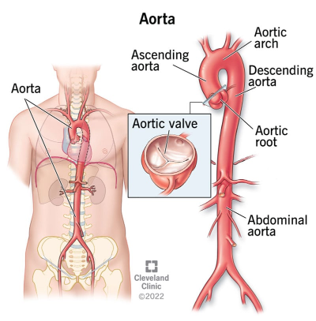
\includegraphics[width=0.4\textwidth]{figures/Intro/Aorta.png}
    \caption[Aorta]{Aorta}
    \label{fig_aorta}
\end{figure}

Aorta segmentation in computerized tomography (CT) scans is important for:
\begin{itemize}
\item Coarctation of the aorta
\item Aortic calcification quantification
\item To guide the segmentation of other central vessels. 
\end{itemize} ~\\

\subsection{Organ Segmentation}
The definition of the organ boundary or organ segmentation is helpful for the orientation and identification of the regions of interest inside the organ during the diagnostic or treatment procedure. Further, it allows the volume estimation of the organ, such as the aorta.

\begin{figure}[ht]
    \centering
    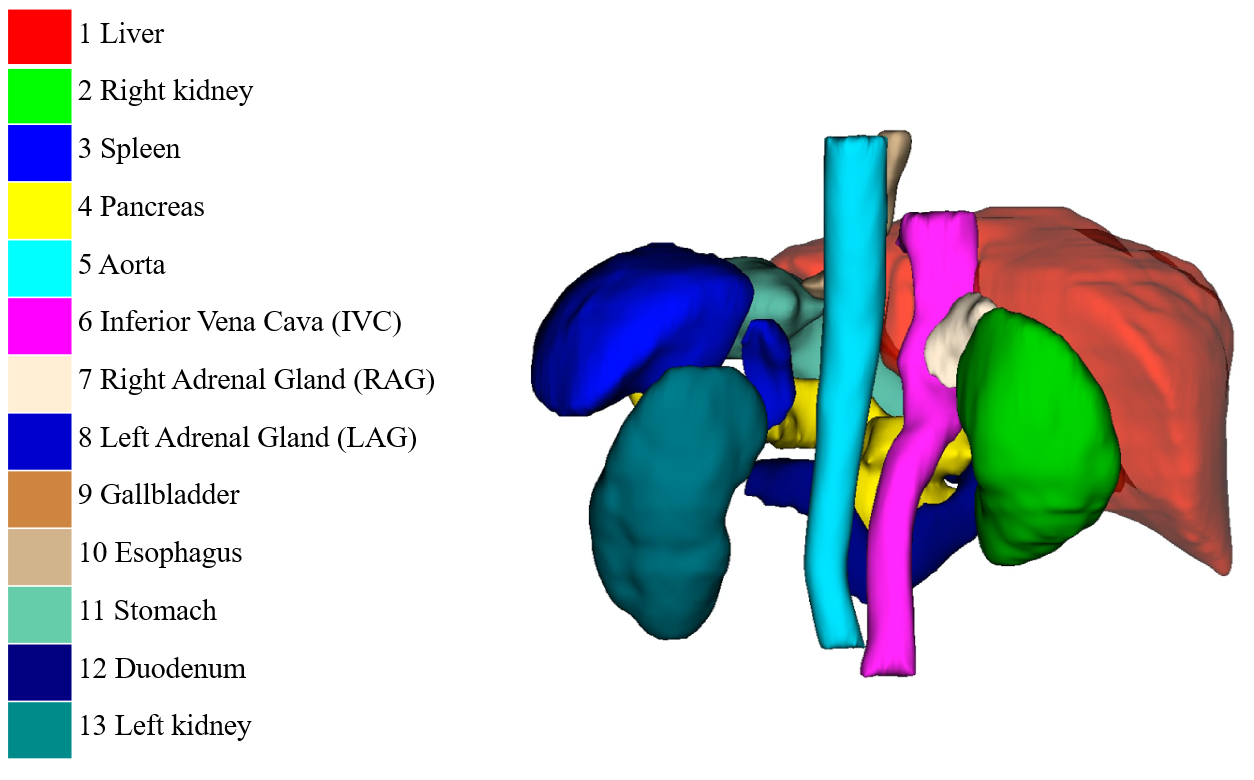
\includegraphics[width=0.7\textwidth]{figures/Intro/segmentation.png}
    \caption[Organ Segmentation]{Organ Segmentation \cite{Ma-2021-AbdomenCT-1K}}
    \label{fig_seg}
\end{figure}

\subsection{Assurance Case}

\begin{figure}[ht]
    \centering
    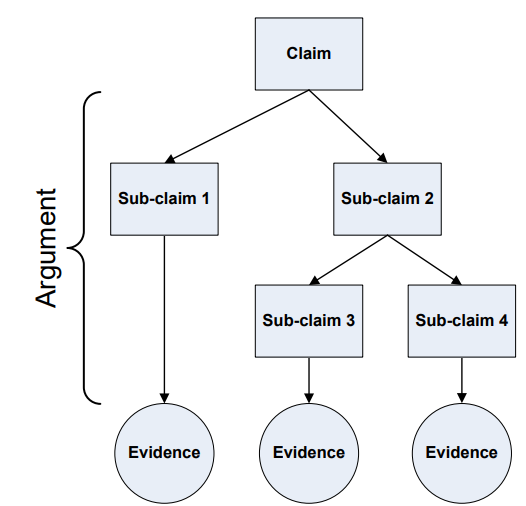
\includegraphics[width=0.45\textwidth]{figures/Intro/ac_diagram.png}
    \caption[Simple Assurance Case Diagram]{Simple Assurance Case Diagram \cite{doi:10.2514/6.2009-1921}}
    \label{fig_ac_diagram}
\end{figure}


An assurance case can be thought of as a specific type of argumentation used in various cases \cite{doi:10.2514/6.2009-1921}. When building an assurance case, you're essentially making a point that specific evidence backs up a particular statement. The fundamental structure is depicted in Figure \ref{fig_ac_diagram}. So, an assurance case essentially boils down to an organized collection of arguments, backed by a body of evidence, that helps validate the belief in a specific claim.

In a practical sense, creating an assurance case involves beginning with a main claim and then breaking it down into smaller claims through a step-by-step process. These smaller claims, at the most bottom, are supported by concrete evidence.


\section{Thesis Outline} \label{TO}

The thesis is organized into three broad parts. In Chapter 2, we introduce our program \progname{} by mentioning the existing methods, the AortaGeomRecon's algorithm overview and step by step  workflow. We explain necessary terms and information to understand how the software functionsfinally, and the 3D Slicer \cite{Kikinis2014} extension module that the user interacts with to get the segmentation result with our algorithm. In Chapter 3, we present our assurance case, some sections of our SRS, Design Documents, Module Guide, Algorithm Review, and a test case we developed for verifying and validating the correctness of program \progname{}. In Chapter 4, future work is proposed and conclusions are drawn based on the developed assurance case, SRS, segmentation algorithm and 3D Slicer module extension.                  
        \setcounter{figure}{0}
        \setcounter{equation}{0}
        \setcounter{table}{0}
        
  \chapter{AortaGeomRecon Research and Development}
This chapter will discuss about the research and development of the \progname{}. \\
AortaGeomRecon stands for Aorta Geometry Reconstruction. The main objective of this software is to semi-automatically build 3D geometry of the Aorta from the patient's chest ct scans.  The existing methods are often involved of extensive manual works with very complex software, with a minimum of 10 minutes of human operator, who is a medical domain expert. \\
The implementation till the date of this report can let the users who have the user characteristics described in SRS get the Aorta 3D geometry with only a few hyperparameters and 2 minutes of execution time. \\


\section{Existing Methods}
There are many segmentation software available to the users, we will discuss the two main methods on two softwares.


\begin{itemize}
\item ITK-Snap\\
ITK-Snap provides a segmentation method that first let user to select multiple voxels with a custom intial size and expanding size within any volume. We refer this method as ``bubble method''.\\
Through many iterations, the voxels expand to fill the entire volume, finally user will need to cut the extra part of the volume. \\
The advantages of the bubble method is that it guarantes to produce a correct the segmentation result. A medical domain expert can manually control the wanted area, and visually observing the segmentation result expanding, shrinking and the user can erase the unwanted part.

The disadvantages of this method is that the operations described above are complicated. Eeasier to say then do, an opeartor who has previous experience building the geometry with this method still needed 20 minutes of manual work building a new aorta geometry. ITK-Snap software can only read VTK file, therefore the chest CT scans are usually DICOM needed a manual conversion before using this software and its segmentation method.

\item 3D Slicer\\
3D Slicer is another well-known medical image processing software for academic. 3D Slicer provides multiple segmentation methods, and one of the quickiest and easiest to use is the intensity based segmentation.\\

This method first let user select a small area that belongs to the wanted area on a 2D plane (Axial, Sagittal, and ). 3D Slicer read the pixels' intensity of the surrounding area, and segment based on the intensity. Any pixels's intensity that are within the range will be segmented as the segmentation result. 

Like the bubble method, this method often reads extra volume, and requires user to cut the unwanted parts. A Youtube video shows an experience user who gets the aorta 3D geometry with 10 minutes of manual works.
\end{itemize}


\section{GitHub and Workflows}
This project uses GitHub for version control. \\
GitHub issues tracker use to keep track the items to work on throughout the development of the project\\
GitHub Project is used for dividing a large issue into smaller tasks, expected date of the completion. This is useful for project management.\\
GitHub Workflow is a great tool for Continuous Integration tests. \\
We uses GitHub Workflow for Linter and Continuous Integration tests. \\

\section{3D Slicer Extension Development}
The project has started with the a simple segmentation algoritm build on the jupyter notebook. When getting a new patient's data, the user will need to investigate the chest ct scans using another software (3D Slicer, ITK-Snap), in order to know the starting voxel and the size crop the volume, and get the index of the aorta seed. This Figure~\ref{fig_aorta_seed} shows an example of the aorta seeds.

\begin{figure}[ht]
    \centering
    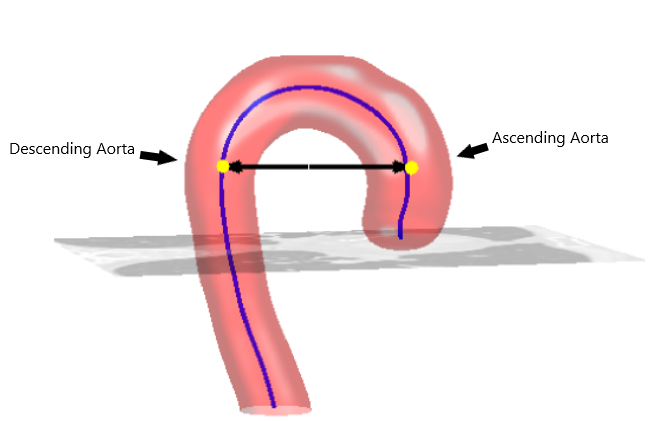
\includegraphics[width=0.6\textwidth]{figures/Sample/Aorta_seeds.png}
    \caption[Single Figure Environment Listed Title]{The aorta seeds}
    \label{fig_aorta_seed}
\end{figure}

In order to improve the usability of the \progname{} (reduce the amount of time for user inputs and execution), we implemented an extension module on 3D Slicer. 

3D Slicer provides very useful modules such as Crop Volume module and Volume Rendering module.

\section{Segmentation Algorithm}

This is a sample chapter

If you need to use quotes, type it ``like this''.


\section{Referencing}
These are some sample references to GAMYGDALA~\citep{popescu2014gamygdala} from 
the \texttt{references.bib} file and state effects of 
cognition~\citep{hudlicka2002time} from the \texttt{references\_another.bib} 
file. These references are not in the same .bib file.
%
%\section{Figures}
%This is a single image figure (Figure~\ref{fig_singleenv}):
%
%\begin{figure}[ht]
%    \centering
%    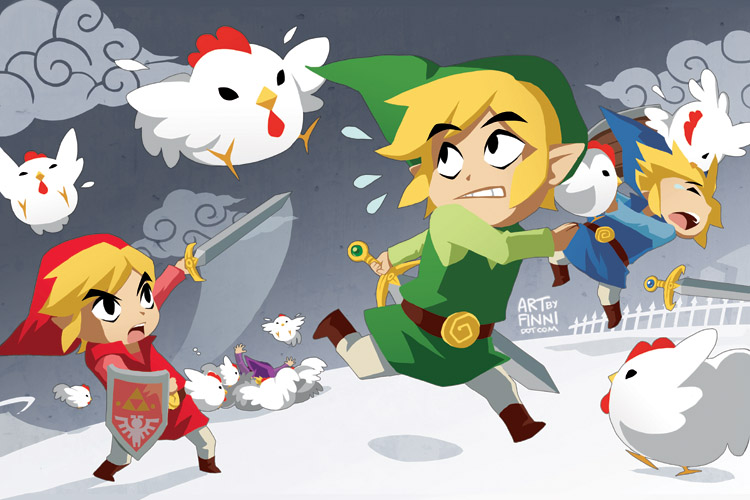
\includegraphics[width=0.6\textwidth]{figures/Sample/tumblr_static_eaceks0rfxsss8o4swscw40wo.jpg}
%    \caption[Single Figure Environment Listed Title]{This is a single figure 
%    environment}
%    \label{fig_singleenv}
%\end{figure}
%
%This is a multi-image figure with a top (Figure~\ref{fig_multienv_1}) and bottom (Figure~\ref{fig_multienv_2}) aligned subfigures:
%
%\begin{figure}[ht]
%	\centering
%	\begin{subfigure}[t]{\textwidth}
%		\centering
%		
%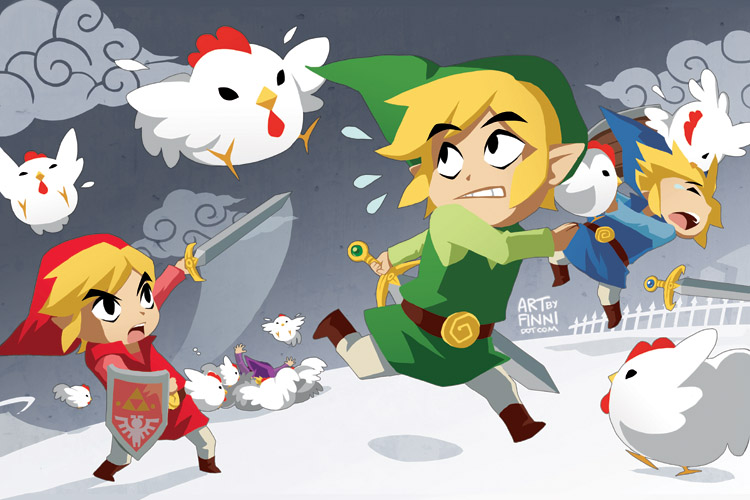
\includegraphics[width=0.7\textwidth]{figures/Sample/tumblr_static_eaceks0rfxsss8o4swscw40wo.jpg}
%		\caption{Figure 1}
%		\label{fig_multienv_1}
%	\end{subfigure}
%	~
%	\begin{subfigure}[t]{\textwidth}
%		\centering
%		
%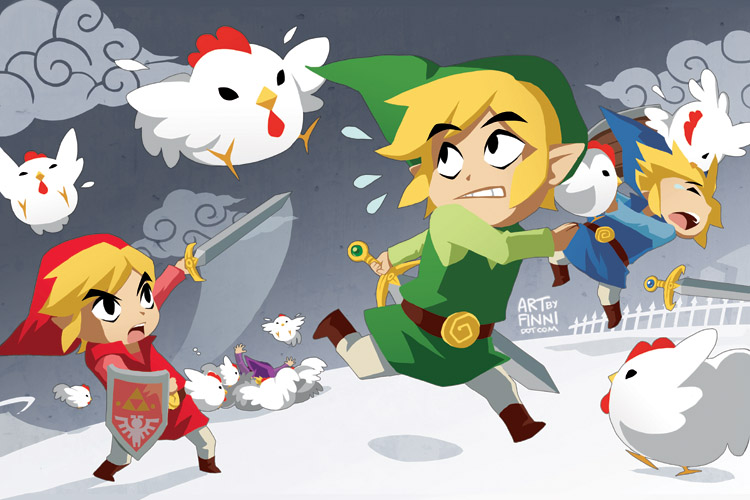
\includegraphics[width=0.7\textwidth]{figures/Sample/tumblr_static_eaceks0rfxsss8o4swscw40wo.jpg}
%		\caption{Figure 2}
%		\label{fig_multienv_2}
%	\end{subfigure}
%	
%	\caption{A Multi-Figure Environment}
%	\label{fig_multienv}
%\end{figure}
%
%\section{Tables}
%
%Here is a sample table (Table~\ref{tab_sample}):
%
%	\begin{table}[ht]
%	\centering
%	\begin{tabular}{ m{0.2\textwidth} m {0.1\textwidth} m{0.15\textwidth} }
%		\toprule
%		A & $\longleftrightarrow$ & B \\
%		C & $\longleftrightarrow$ & D \\
%		\bottomrule	
%	\end{tabular}	
%	\caption{A sample table}	
%	\label{tab_sample}
%\end{table}
%
%\subsection{Long Tables}
%A sample long table is shown in Appendix~\ref{appendix_b}.
%
%\section{Equations}
%
%Here is a sample equation (Equation~\ref{eq_lineslope}):
%
%\begin{equation} \label{eq_lineslope}
%	y = mx + b
%\end{equation}                  
       \setcounter{figure}{0}
       \setcounter{equation}{0}
       \setcounter{table}{0}

  \chapter{Assurance Cases and Selected Evidence for AortaGeomRecon}

\section{Assurance Case Development}

\section{Assurance Case for Software Specification Requirements}

\begin{itemize}
\item \citep{SRS}
\item Goals
\item Assumptions
\item Data Definitions
\item Instance Model
\item Functional Requirements
\item Non-Functional Requirements
\item Traceability Matrix Between Different Sections
\item Traceability Matrix Between Requirements and Other Sections
\end{itemize}

\section{Assurance Case for Implementation}
\begin{itemize}
\item Design Document
\begin{itemize}
\item Sphinx - Python Documentation Generator
\item Comments in the source code
\item Algorithm Overview - Explanation and Program Workflow
\item Glossary
\end{itemize}
\item Module Guide
\begin{itemize}
\item Traceability Matrix between Modules and Requirements
\item Traceability Matrix between Modules and Source Code
\end{itemize}

\item Test Case
\begin{itemize}
\item GitHub Workflow
\item Continuous Integration tests
\begin{itemize}
\item build ``Ground Truth Data''
\item Steps
\item Coverage
\end{itemize}
\end{itemize}

\end{itemize}

\section{Algorithm Review}
\begin{itemize}
\item Python Spyder IDE - Data Visualization and Debugging tool
\item Algorithm Review with Kailin Chu
\item Algorithm Review with Dr. Dean Inglis
\end{itemize}


%\section{Referencing}
%These are some sample references to GAMYGDALA~\citep{popescu2014gamygdala} from 
%the \texttt{references.bib} file and state effects of 
%cognition~\citep{hudlicka2002time} from the \texttt{references\_another.bib} 
%file. These references are not in the same .bib file.
%
%\section{Figures}
%This is a single image figure (Figure~\ref{fig_singleenv}):
%
%\begin{figure}[ht]
%    \centering
%    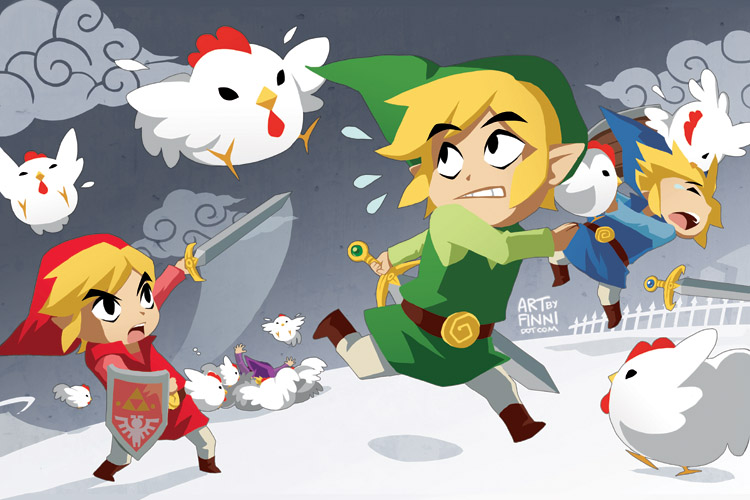
\includegraphics[width=0.6\textwidth]{figures/Sample/tumblr_static_eaceks0rfxsss8o4swscw40wo.jpg}
%    \caption[Single Figure Environment Listed Title]{This is a single figure 
%    environment}
%    \label{fig_singleenv}
%\end{figure}
%
%This is a multi-image figure with a top (Figure~\ref{fig_multienv_1}) and bottom (Figure~\ref{fig_multienv_2}) aligned subfigures:
%
%\begin{figure}[ht]
%	\centering
%	\begin{subfigure}[t]{\textwidth}
%		\centering
%		
%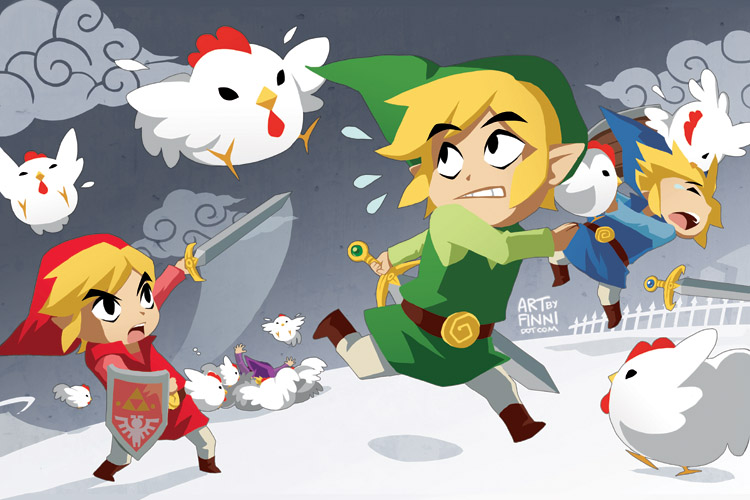
\includegraphics[width=0.7\textwidth]{figures/Sample/tumblr_static_eaceks0rfxsss8o4swscw40wo.jpg}
%		\caption{Figure 1}
%		\label{fig_multienv_1}
%	\end{subfigure}
%	~
%	\begin{subfigure}[t]{\textwidth}
%		\centering
%		
%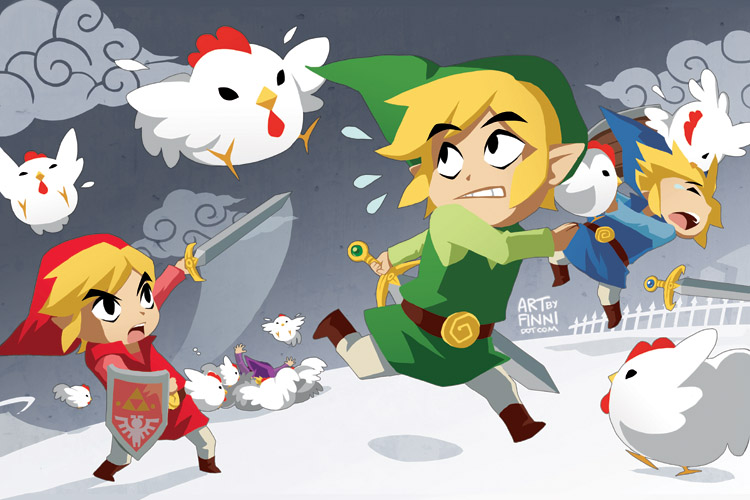
\includegraphics[width=0.7\textwidth]{figures/Sample/tumblr_static_eaceks0rfxsss8o4swscw40wo.jpg}
%		\caption{Figure 2}
%		\label{fig_multienv_2}
%	\end{subfigure}
%	
%	\caption{A Multi-Figure Environment}
%	\label{fig_multienv}
%\end{figure}
%
%\section{Tables}
%
%Here is a sample table (Table~\ref{tab_sample}):
%
%	\begin{table}[ht]
%	\centering
%	\begin{tabular}{ m{0.2\textwidth} m {0.1\textwidth} m{0.15\textwidth} }
%		\toprule
%		A & $\longleftrightarrow$ & B \\
%		C & $\longleftrightarrow$ & D \\
%		\bottomrule	
%	\end{tabular}	
%	\caption{A sample table}	
%	\label{tab_sample}
%\end{table}
%
%\subsection{Long Tables}
%A sample long table is shown in Appendix~\ref{appendix_b}.
%
%\section{Equations}
%
%Here is a sample equation (Equation~\ref{eq_lineslope}):
%
%\begin{equation} \label{eq_lineslope}
%	y = mx + b
%\end{equation}                  
       \setcounter{figure}{0}
       \setcounter{equation}{0}
       \setcounter{table}{0}

  \chapter{Conclusion and Future Works}

This chapter provides a summary of the thesis (Section \ref{thesis_sum}), the challenges (Section \ref{challenge}), and the future work (Section \ref{fw}).

\section{Thesis Summary}\label{thesis_sum}

This project developed software as a 3D Slicer extension to semi-automatically extract a 3D geometry of the aorta. To build confidence in the software, we applied assurance case arguments. The project started from a Jupyter Notebook program as left by a previous student. With this as a starting point, we explored what changes to the documentation, design, implementation and verification activities are necessary for the assurance case. We did the following tasks in the chronological order for the evidence supporting our assurance case:

 \begin{myEnumerate}
\item Build the continuous integration infrastructure with GitHub Actions for the algorithm. This allows us to update the algorithm, and making sure that the valid update is at least as good as the previous version. 
\item A linter is set up as part of the continuous integration test to ensure the program's readability by enforcing the PEP8 standard.
\item Draft our Software Requirements Specification (SRS).
\item Draft our high-level design Module Guide (MG).
\item Build a graphical user interface (GUI) because the existing approach had poor usability since it required using other software to determine the necessary parameters and then editing the code.
\item Use 3D Slicer as the platform to implement our GUI because it is modular, and it provides useful features such as Volume Rendering, volume visualization, Crop Volume and reading coordinate on a volume interactively.
\item Build assurance cases in Goal Structuring Notation with the bottom-up approaches. We gather our existing evidence, and explore new implementation requirement for the new evidence.
\item Write user instructions on GitHub README to instruct the user on how to use AGR correctly.
\item Film and post a user instructions video with voice over to provide a clear and direct user instructions.
\item Build a detailed design document and hosted on a web server.
\item Scheduled Code Review with Kailin Chu.
\item Scheduled Algorithm Review with Dr. Dean Inglis.
\item Finalize our SRS, MG, and assurance case. 
\end{myEnumerate}

It is worth mentioning that GitHub Issues, Discussions, and Pull requests are used throughout the development of the software for the project management. Dr. Spencer Smith and I were able to keep up good communication through the use of the GitHub features. Finally, weekly and bi-weekly meetings were scheduled to help us communicate efficiently.

\section{Challenge}\label{challenge}
In the course of this project, we have summarized a list of challenges. The first challenge was looking for an ideal platform to develop \progname{} software. At the beginning of the project, we wanted to develop our own software without any external platform. Until the point where we saw that it is not feasible to build from scratch a volume visualization system like the one provided by 3D Slicer, time and efforts were wasted in designing a UI, finding the right tool to build the UI, etc. 

The second challenge is that 3D Slicer itself is a very complex software, the development resource is limited and difficult to understand. Some features provided by 3D Slicer are not obvious until you have searched through its built-in module list, which has approximately 30 modules.

Another obstacle that we had is having a domain expert to examine the quality of our segmentation result. This medical software's intended user is a university student studying in medical science or medicine, who needs to get an aorta's image or quantified volume. Throughout the development of the \progname{}, we did not have an intended user or a domain expert to review our software. However, Dr. Spencer Smith and I were also lacking the knowledge and do not know the expectation of the intended user. This causes ambiguity to specify the true requirements of AGR, until we were able to spend time with Dr. Inglis.

Finally, it was very challenging to understand assurance cases within a limited amount of time. Gathering the evidences and supporting our arguments was not in my imagination at the beginning of the project. Without truly understanding our goals for the project, I was not certain what I was really doing. Once we have several pieces linking together, I was able to finally understand and make my efforts in the right direction. 

\section{Lessons Learned}\label{ll}
After reviewing all available evidence and constructing the assurance case for AortaGeomRecon, we have compiled a list of lessons learned that could prove valuable to those seeking to develop assurance cases for research software.

When crafting the Software Requirement Specification document, it is advisable to describe our data definitions and instance models using commonly accepted mathematical notation. Since our target audience includes domain experts who may not be software developers, it is crucial not to represent instance models using pseudocode. Utilizing mathematical notation also facilitates the review process for domain experts, ensuring completeness, correctness, and consistency within the document.

The traceability matrix offers a transparent means for illustrating the relationships between various levels of abstractions. First and foremost, the traceability matrix enables other developers to verify whether the modules outlined in the Module Guide genuinely serve a purpose in fulfilling specific requirements. Furthermore, by establishing a correspondence between the modules and the source code, it allows for the verification of whether the implementation indeed provides the functionality described in the modules within the Module Guide.

Despite all the operational assumptions detailed in the documentation, it is essential to include a warning message to caution users about the proper use of this software. This is a requirement for all critical software, including medical image processing software, as diagnoses could rely on the generated results, potentially impacting a patient's well-being. When the software can only guarantee expected output under specific assumptions, we trust users not to violate these assumptions, and we have a responsibility to remind them of their duties.

Finally, we have learned how to conduct a code walkthrough, a code review, and an algorithm review to verify the implementation's correctness. To start this process effectively, it's advisable to conduct a code walkthrough alongside a software developer who recently worked on the same segment of the implementation. This ensures that the collaborator still holds a fresh memory of significant software decisions and expected output, allowing for meaningful discussions about how the implementation achieved these results.

Code and algorithm reviews have quickly provided insights into which portions of the implementation can remain untouched and where improvements can be made. During our code review with Kailin Chu, we identified a step in the segmentation algorithm implemented through trial and error. Collaboratively, we brainstormed ways to enhance this step, resulting in a significant improvement in our segmentation algorithm. In our algorithm review with Dr. Dean Inglis, he shared industry-standard methodologies for image segmentation and introduced a new segmentation method, which can reduce the execution time and eliminate some hyperparameters when applied to our algorithm.


\section{Future Work}\label{fw}

In this section, we discuss some possible future work that can make \progname{} better. The first improvement can be done in the segmentation algorithm, and the second improvement involve completing our assurance case.

\subsection{Segmentation Algorithm}

In this section, we discuss the possible future work related to the segmentation algorithm. Section \ref{new_seg} discusses a similar segmentation algorithm that requires fewer hyperparameters. Section \ref{inglis_seg} discusses a method that eliminates the use of a verification step described in our segmentation algorithm.

\subsubsection{3D Level Set Approach}\label{new_seg}
An improved segmentation algorithm \cite{6346433} is available. Like our segmentation algorithm, this algorithm also needs a cropped volume and the aorta seeds to perform segmentation. However, it requires fewer hyperparameters, such as the parameters for SimpleITK's ThresholdSegmentationLevelSetsFilter. Using this algorithm will reduce the problem of user inputs, which will help to build the evidence for E\_GA.1 discussed in Figure~\ref{fig_agr_ac_ga}.

\subsubsection{Oblique Plane Segmentation}\label{inglis_seg}
This algorithm is proposed by Dr. Dean Inglis discussed during our Algorithm Review meeting. This algorithm is based on the assumption that a healthy aorta should have reasonably uniform diameter along its length. With an initial center coordinate seed and the corresponding diameter, the algorithm can segment the aortic arch through an Oblique Plane. Figure~\ref{fig_oblique} shows the double oblique plane in the ascending aorta, and aortic arch.

\begin{figure}[H]
    \centering
    \fbox{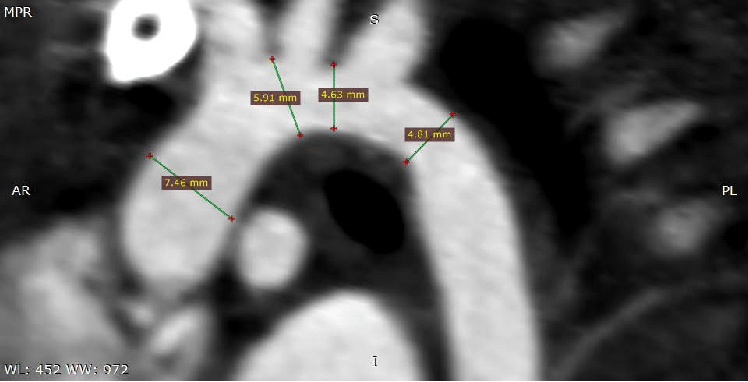
\includegraphics[width=0.8\textwidth]{figures/Conclusion/Ascending-aorta-aortic-arch-and-isthmic-region-in-a-double-oblique-plane-in-a.png}}
    \caption[Aorta Double Oblique Plane]{Aorta Double Oblique Plane}
    \label{fig_oblique}
\end{figure}

Successfully applying this algorithm will eliminate the need of verifying the segmentation result, discussed in Section \ref{stopping_condition}.

\subsection{Assurance Case}

There is room for improvements on the arguments of the requirements of \progname{}. The scope of our project was to explore the breadth of the work needed for an AC. The next step would be to go into the depth where necessary. The correctness of the document is reviewed and approved by a domain expert, where there should be evidences that can support the argument. The evidence for  E\_GA.1 discussed in Figure~\ref{fig_agr_ac_ga} is missing because we did not have the time to complete our Verification and Validation Plan (VnV). The VnV should include the test report, an evidence for E\_GA.1, that will indicate if \progname{} throws an exception when the inputs do not meet one or more of the assumptions, with a message that clearly states the reason.
        \setcounter{figure}{0}
        \setcounter{equation}{0}
        \setcounter{table}{0}

\begin{appendix}
\chapter{Software Requirements Specification for \progname{}}\label{SRS}

\includepdf[pages=-]{../SRS/SRS.pdf}
\chapter{Module Guide for \progname{}}\label{MG}
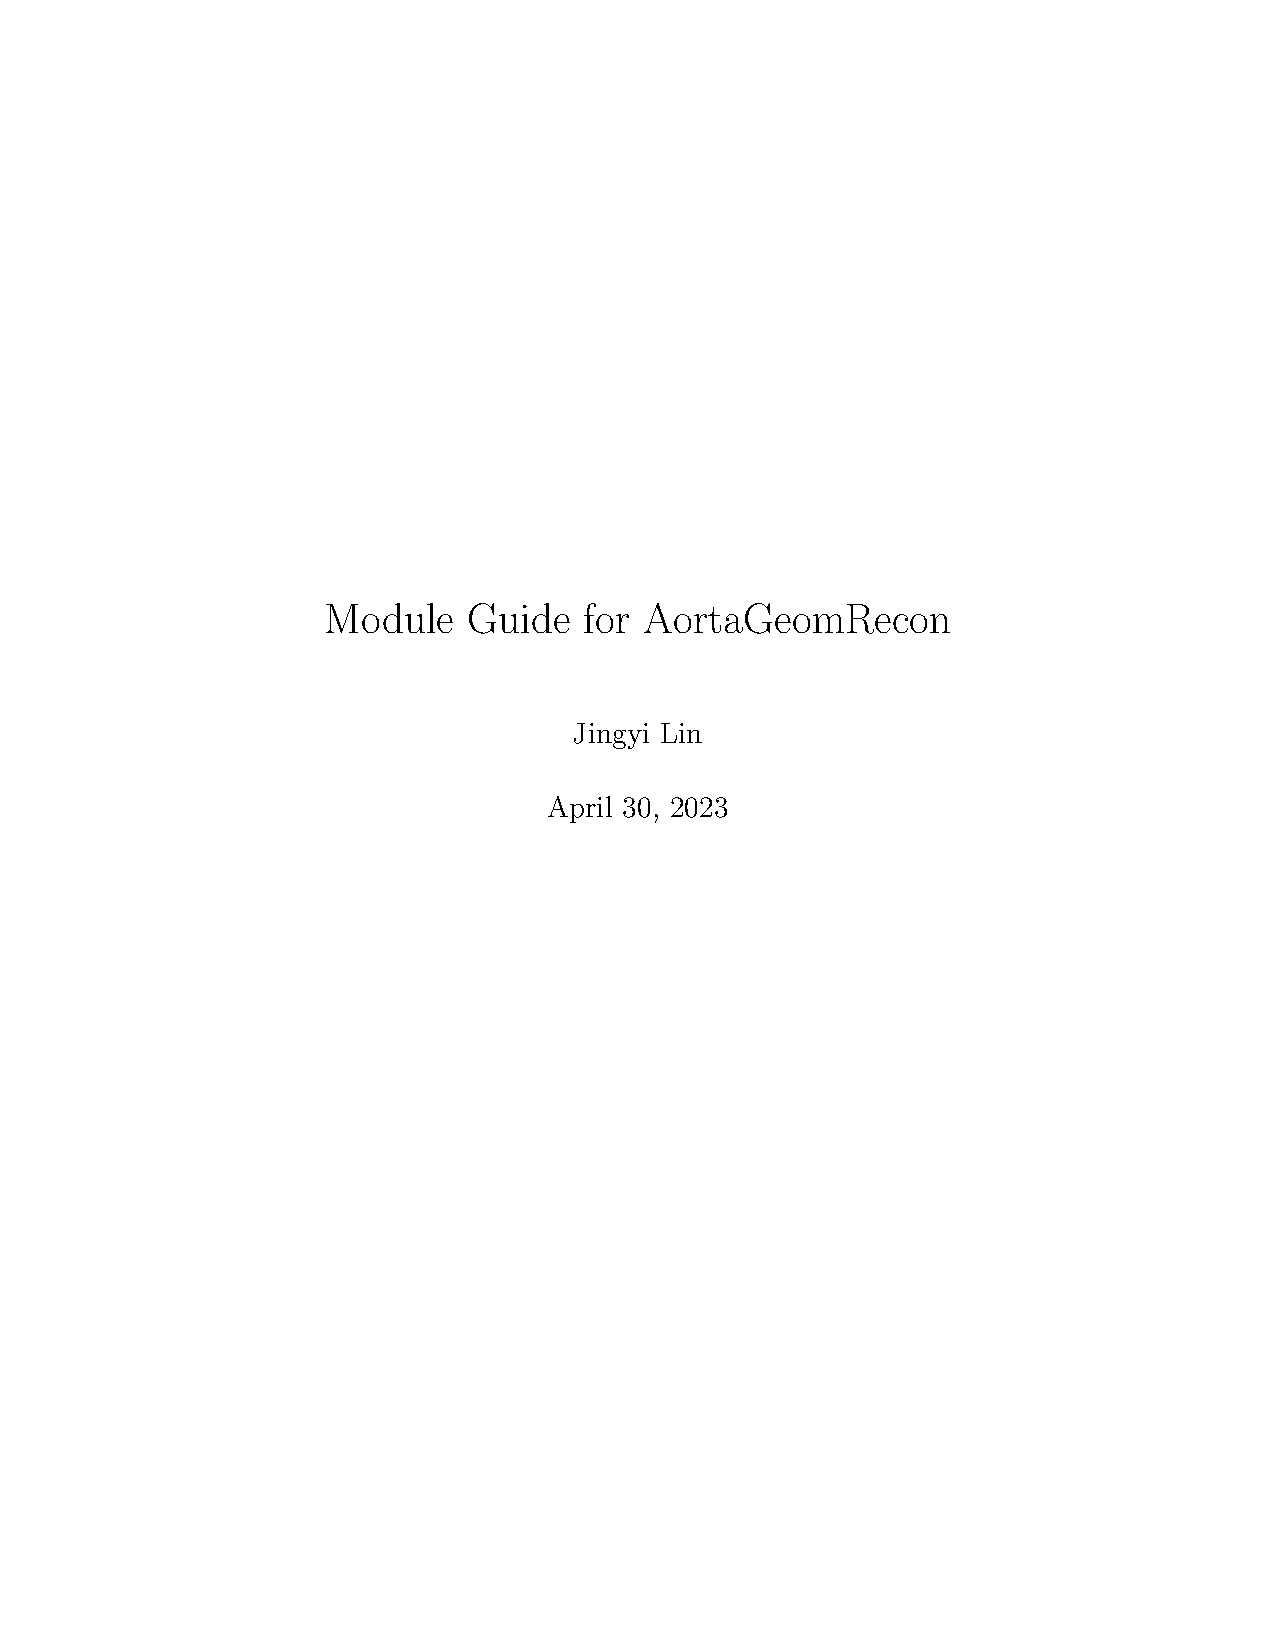
\includepdf[pages=-]{../Design/MG/MG.pdf}
%    \chapter{Your Appendix}
\label{appendix_a}

Your appendix goes here.

%        \setcounter{figure}{0}
%        \setcounter{equation}{0}	
%        \setcounter{table}{0}

%    \chapter{Long Tables}
\label{appendix_b}

%This appendix demonstrates the use of a long table that spans multiple pages.
%
%\begin{center}
%\begin{longtable}{P{3cm}P{3cm}P{2.5cm}P{3.5cm}}
%\toprule
%\hline
%\textbf{Col A} & \textbf{Col B} & \textbf{Col C} & \textbf{Col D} \\ \midrule
%
%\endfirsthead
%\multicolumn{4}{c}{\textit{Continued from previous page}} \\ \hline
%\textbf{Col A} & \textbf{Col B} & \textbf{Col C} & \textbf{Col D} \\ \hline
%\endhead
%\hline \multicolumn{4}{r}{\textit{Continued on the next page}} \\
%\endfoot
%\hline
%\endlastfoot
%
%A & B & C & D \\ \midrule
%
%A & B & C & D \\ \midrule
%
%A & B & C & D \\ \midrule
%
%A & B & C & D \\ \midrule
%
%A & B & C & D \\ \midrule
%
%A & B & C & D \\ \midrule
%
%A & B & C & D \\ \midrule
%
%A & B & C & D \\ \midrule
%
%A & B & C & D \\ \midrule
%
%A & B & C & D \\ \midrule
%
%A & B & C & D \\ \midrule
%
%A & B & C & D \\ \midrule
%
%A & B & C & D \\ \midrule
%
%A & B & C & D \\ \midrule
%
%A & B & C & D \\ \midrule
%
%A & B & C & D \\ \midrule
%
%A & B & C & D \\ \midrule
%
%A & B & C & D \\ \midrule
%
%A & B & C & D \\ \midrule
%
%A & B & C & D \\ \midrule
%
%\hline
%\end{longtable}
%\end{center}

%        \setcounter{figure}{0}
%        \setcounter{equation}{0}
%        \setcounter{table}{0}
\end{appendix}

% The bibliography is set up to allow for multiple bib files
\bibliographystyle{acm}
\bibliography{references,references_another}

\label{NumDocumentPages}

\end{document}
% ********************************
